\ifx\fulldocument\undefined
\documentclass[aspectratio=169]{beamer}
% \usetheme{sdr}
\graphicspath{{./tex/imgs/}}

\usepackage[utf8]{inputenc}

\title{Programmiamo Umanoidi!}
\subtitle{}
\author{Lorenzo Leonardini}
\institute{Scuola di Robotica}
\date{\today}

\begin{document}

\begin{frame}
	\titlepage
\end{frame}

\section{Che cos'è NAO}
\subsection{Caratteristiche}
\subsection{Movimento}
\subsection{Utilizzi}
\subsection{Software}
\section{Choregraphe}
\section{Primo programma}
\section{NAO Actor Studio}
\section{NAO In The Store}

\AtBeginSection[]
{
\begin{frame}{Indice}
\tableofcontents[currentsection]
\end{frame}
}
\fi

\section{NAO Vision}

\begin{frame}
\frametitle{NAO Vision}
\begin{itemize}
	\item<1-> La visione artificiale(\textit{Computer Vision}) ha lo scopo di riprodurre la vista umana
	\item<2-> "Visione" intende l'interpretazione del contenuto di un'immagine
\end{itemize}
\end{frame}

\begin{frame}
\frametitle{NAO Vision}\
Compiti tipici:
\begin{itemize}
	\item<2-> \textit{Recognition}: riconoscere un oggetto generale (hey c'è una faccia!)
	\item<3-> \textit{Identification}: identificare un oggetto specifico (hey quella è la faccia di Tizio!)
\end{itemize}
\end{frame}

\begin{frame}
\frametitle{NAO Vision}
\begin{columns}
	\column{0.5\textwidth}
		Cosa può fare NAO:
		\begin{itemize}
			\item<2-> Riconoscere facce e identificare persone
			\item<3-> Riconoscere una pallina rossa
			\item<4-> Riconoscere e leggere i NAOMark
			\item<5-> Riconoscere oggetti personalizzati
		\end{itemize}
	\column{0.5\textwidth}
		\begin{figure}[ht]
		\begin{center}
		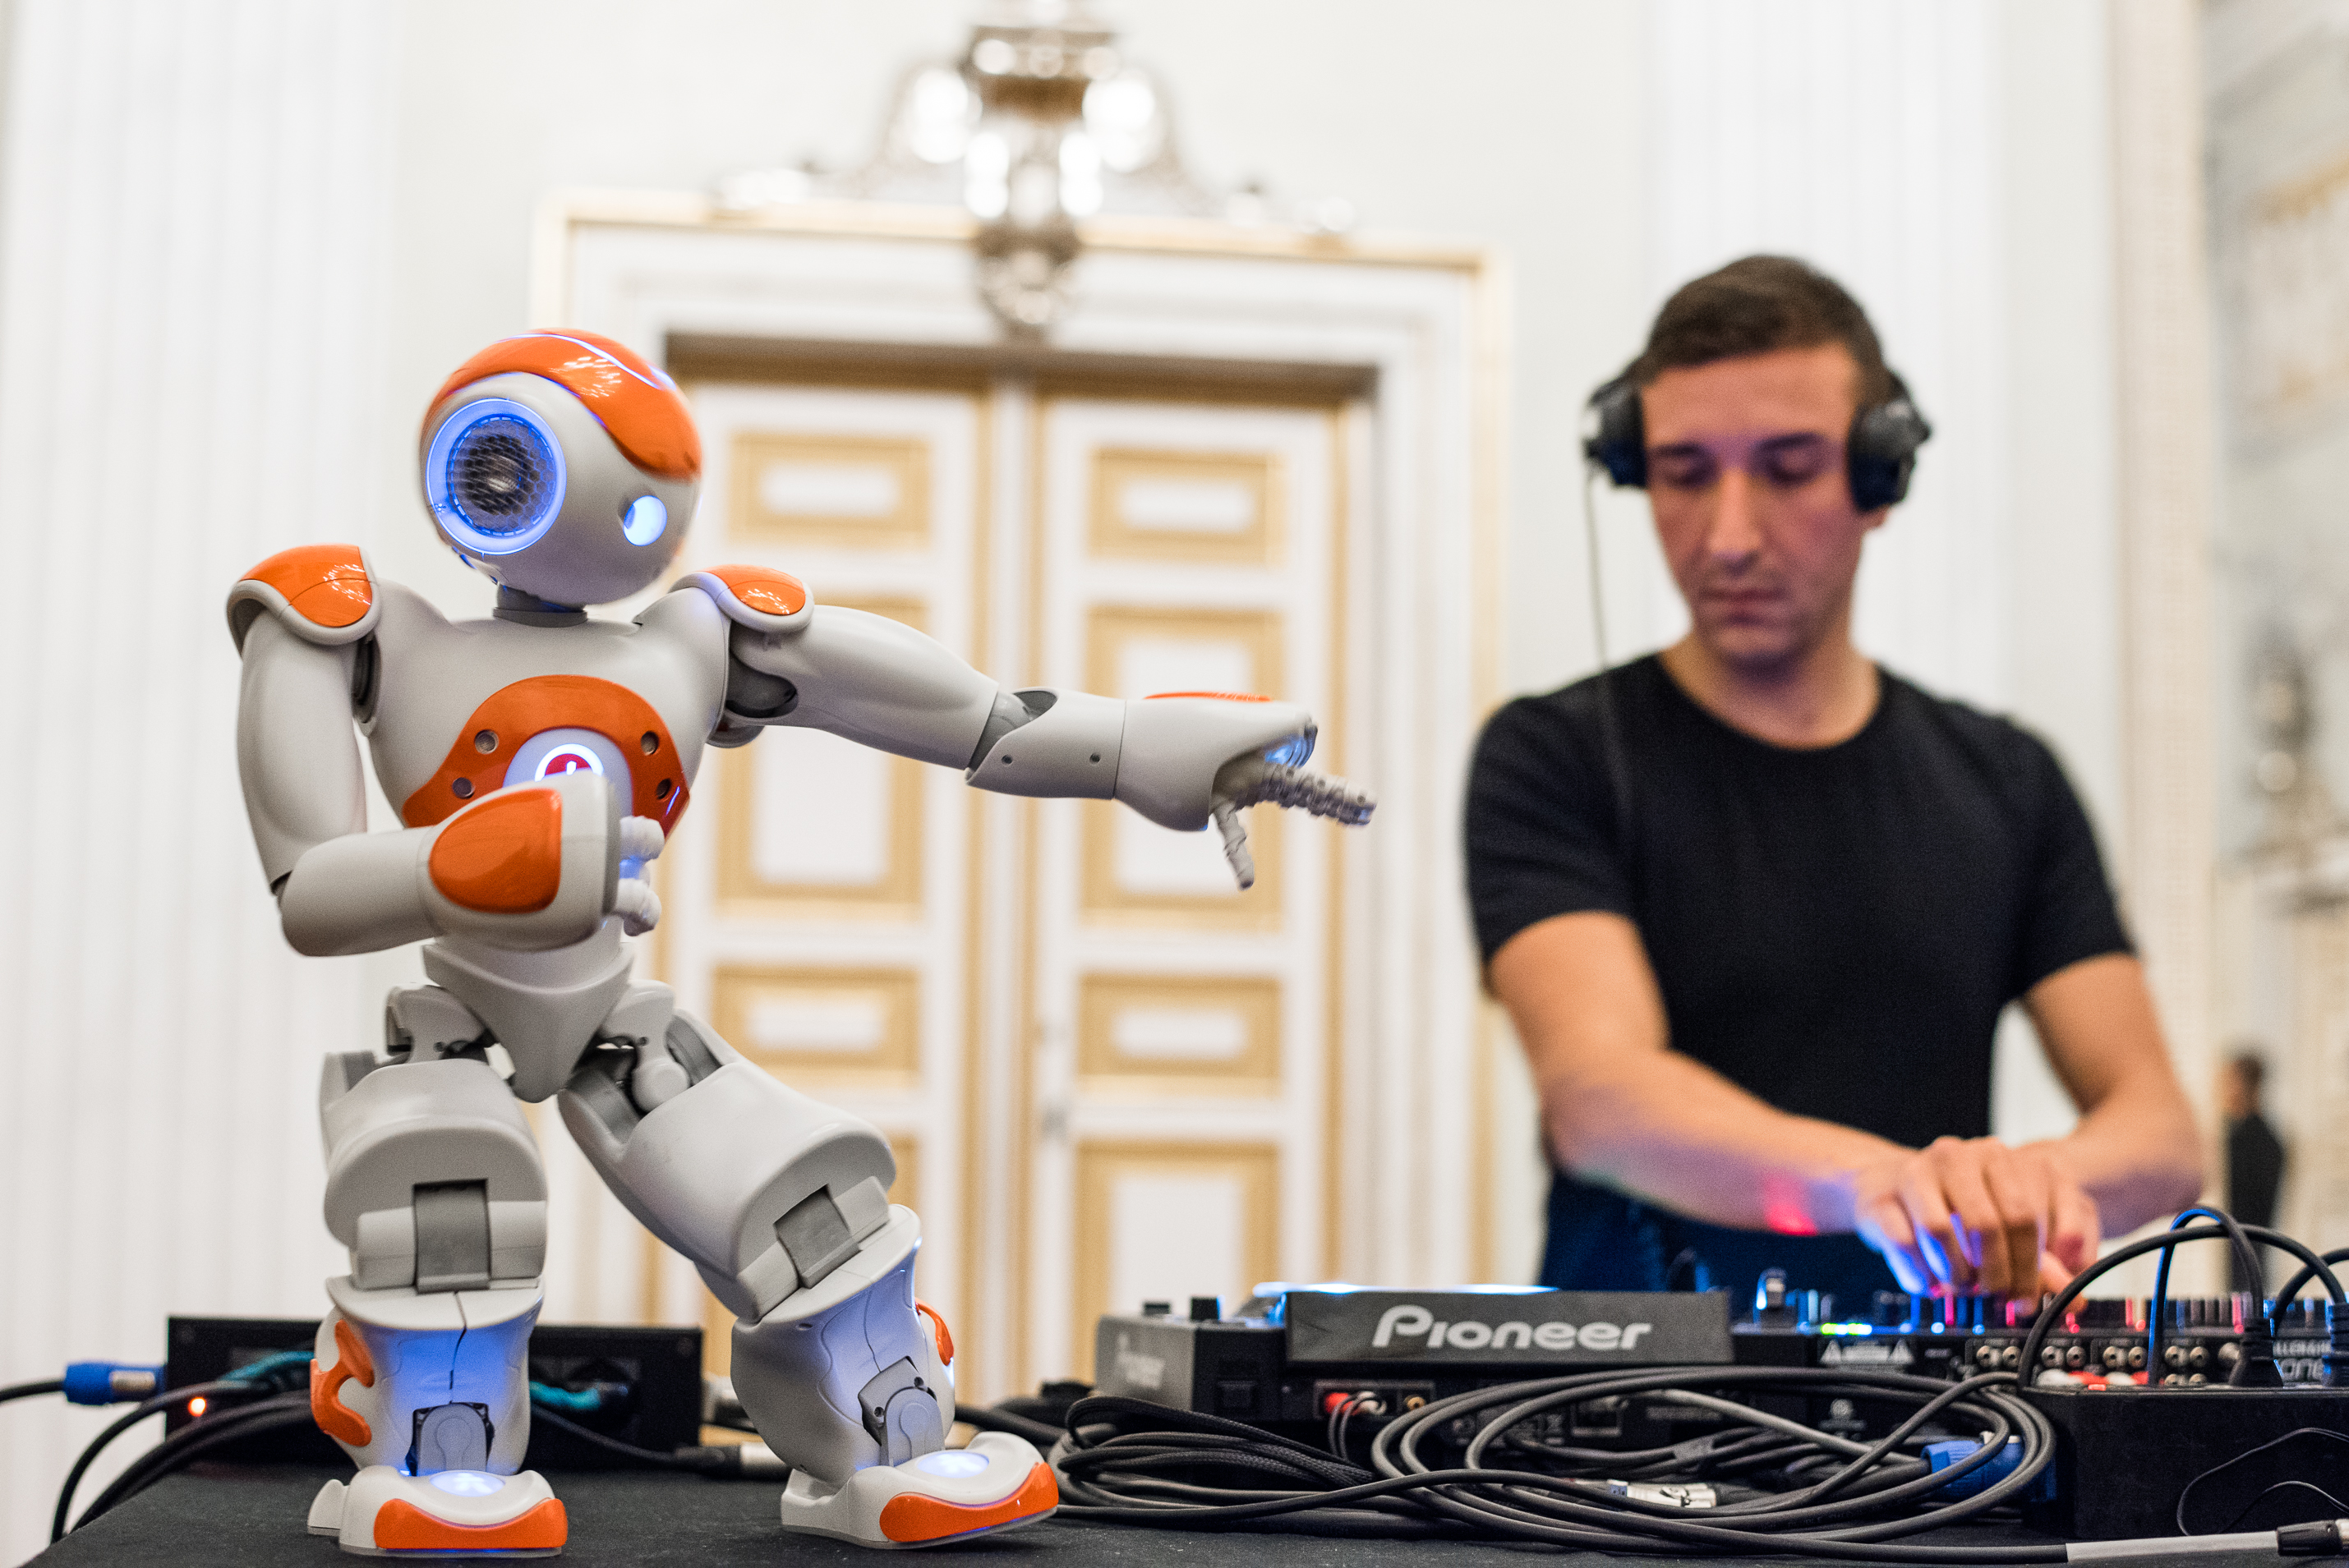
\includegraphics[width=.9\textwidth]{nao7}<1->
		\end{center}
		\end{figure}
	\end{columns}
\end{frame}

\begin{frame}
\frametitle{NAO Vision}
Tracking:
\begin{itemize}
	\item<2-> NAO può seguire gli oggetti riconosciuti
	\item<3-> Seguire vuol dire con lo sguardo ma anche con il corpo o muovendosi incontro
\end{itemize}
\end{frame}

\ifx\fulldocument\undefined
\end{document}
\fi
